\chapter[SCP-064 伪冯诺依曼建筑]{
    SCP-064 Flawed von Neumann Structure\\
    SCP-064 伪冯诺依曼建筑
}

\label{chap:SCP-064}

\begin{figure}[H]
    \centering
    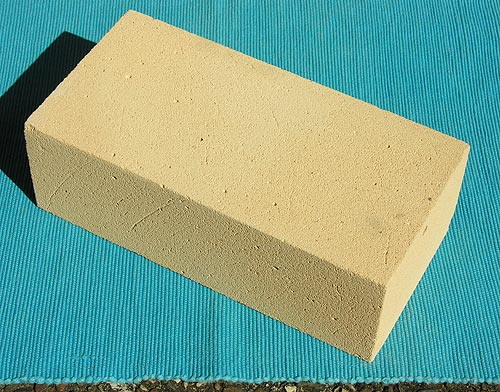
\includegraphics[width=0.5\linewidth]{images/SCP.064.jpg}
    \caption*{SCP-064}
\end{figure}

\bb{项目编号:}SCP-064

\bb{项目等级:}Safe

\bb{特殊收容措施:}SCP-064应被保管于一个合适的远程监控区域以供观察。目前的目标是建立一个关于此物体行为规律的几何模型并且观察这些规律根据地点和土壤成分不同而产生的变化。某些位于戈壁沙漠,澳大利亚腹地的地点以及数块分散在全球的盐碱地都被纳入考虑以期将来的实验。SCP-064的目前位置允许所有安保级别三级以下的人员进入。一旦生长结束,野外工作队将要把建筑物的尺寸,形状和成分归档,并且将对象转移至一个新的地区。

\bb{描述:}SCP-064是一块亮棕色的陶土砖,主要由硅氧化物和一些有机质组成。对象重1.6千克,尺寸量得为10cmX6cmX20cm。其表面光滑平整,有一些细小的碎屑。大体上对象看起来和用于建筑的固体砖块非常相似。

当被放在一块平整开阔的柔软土地上时,SCP-064会开始通过未知机能自我复制。近距离观察发现有何原对象形状一样的不规则的硅纤维晶体形成,随后其以一种基于土壤的混合物填充并且固化自身直到达到一个合适的质量。这个过程和真菌菌丝体的传播有些相似,用微小的根部结构从紧邻的土壤里“发掘”矿物质。在最理想状态下(土壤成分约含90\%的二氧化硅{[}SiO\textsubscript{2}]),需要大概七十分钟以产生一块完整的新砖。

在一块广阔的土地上,SCP-064会建造一座非常复杂但是理论上稳定的独立砖石建筑,包括地板和天花板。过去的观察表明这些建筑可以达到十二角星的形状,周长10千米,重量可观。然而,这些都是推测,因为建筑一旦接触一个重大障碍物,据观察包括所有质量在10千克之上的固体物体时,生长就会停止。有趣的是,建筑的生长有一种特别的基本方向规律,那就是SCP-064总是在最北方并且在最底层。

建筑必须在接连SCP-064时才会成长。一旦取走SCP-064,建筑会开始崩溃,所有的次级砖块都会以与出现时相同的速度崩碎成为尘土。在二十分钟内放回SCP-064可以阻止崩溃并且使成长继续;超过这个时限,崩溃过程就再不可逆。

SCP-064是在20██年四月偶然发现的。当对安第斯山脉的一块高架高原进行卫星观测时,一个摄像机操作者注意到一座建筑正在明显的生长。从建筑的外部生长方向(当回收时生长已经停止)推断出了对象大约的位置后,野外工作队通过SCP-064和富含来自当地土壤中的氧化铁的次级砖之间颜色的不同发现了对象。对于原始地点的完整发掘工作正在进行中以确定对象的文化和技术起源。
